\newpage
\section{QuizziPedia::Front-End}
\label{QuizziPedia::Front-End}
\begin{figure}[ht]
	\centering
	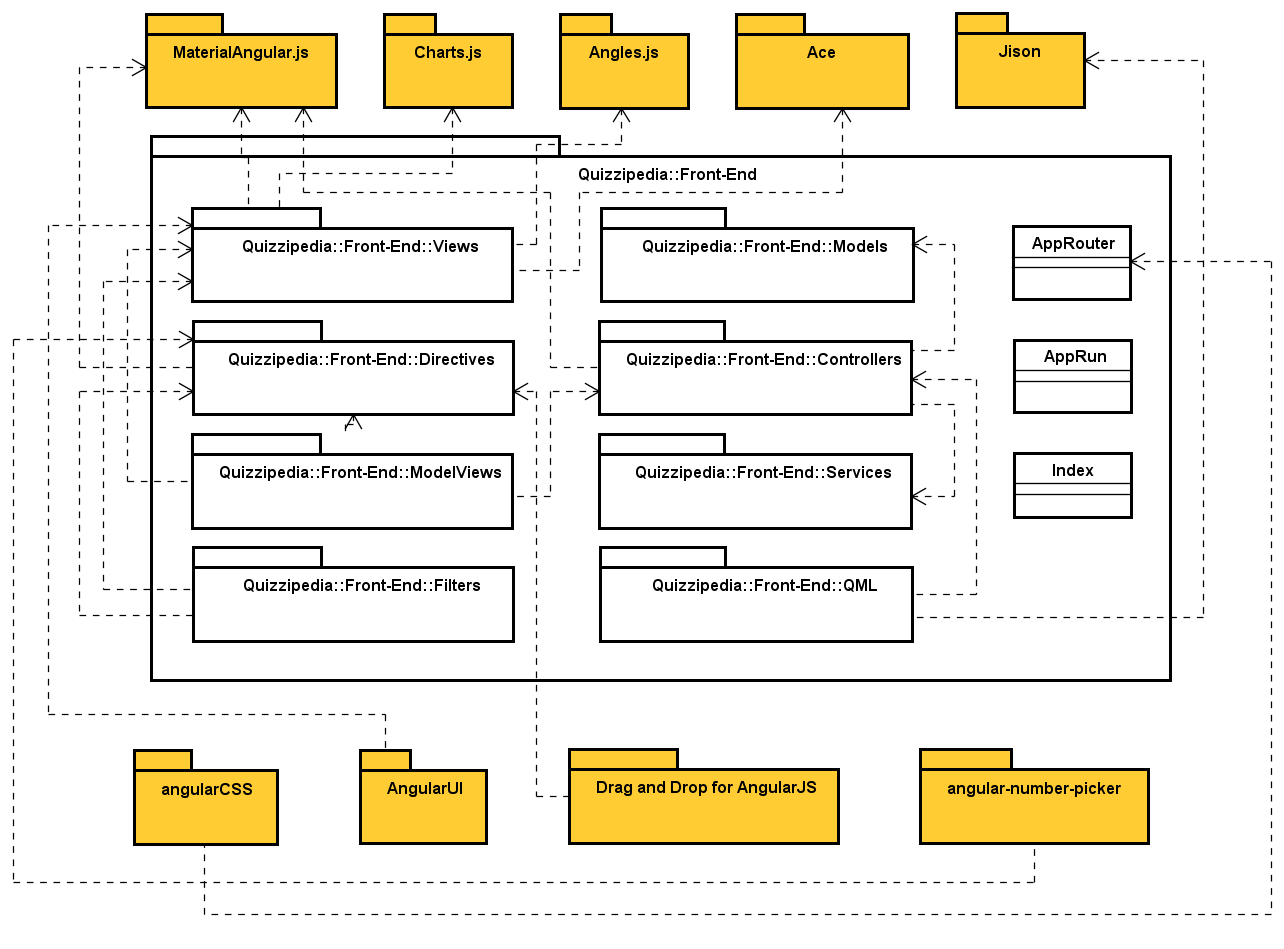
\includegraphics[scale=0.40]{UML/Package/QuizziPedia_Front-end.png}
	\caption{QuizziPedia::Front-End}
\end{figure}
\FloatBarrier
\begin{itemize}
	\item \textbf{Descrizione}: \textit{package\ped{G}} contenente le componenti front-end dell'applicazione;
	\item \textbf{Package contenuti}:
	\begin{itemize}
		\item \texttt{Views}: \textit{package\ped{G}} contenente le \textit{views\ped{G}} front-end dell'applicazione;
		\item \texttt{Controllers}: \textit{package\ped{G}} contenente i \textit{controllers\ped{G}} front-end dell'applicazione;
		\item \texttt{Services}: \textit{package\ped{G}} contenente i \textit{services\ped{G}} front-end dell'applicazione;
		\item \texttt{Models}: \textit{package\ped{G}} contenente le classi che definiscono la business logic dell'applicazione;
		\item \texttt{Directives}: \textit{package\ped{G}} contenente le \textit{directives\ped{G}} front-end dell'applicazione.
	\end{itemize}
	\item \textbf{Classi contenute}:
	\begin{itemize}
		\item \texttt{Index}: \textit{view\ped{G}} generale dell'applicazione. Contiene gli elementi che saranno presenti in ogni pagina dell'applicazione;
		\item \texttt{AppRun}: classe che verifica se l'utente sia autenticato e che abbia le giuste autorizzazioni per la pagina in cui si trova;
		\item \texttt{AppRouter}: classe che gestisce i routes dell'applicazione, utilizza il servizio \$routeProvider per associare ad ogni route un \textit{controller\ped{G}} e una \textit{view\ped{G}}.
	\end{itemize}
\end{itemize}

\newpage
\subsection{QuizziPedia::Front-End::Views}

\label{QuizziPedia::Front-End::Views}
\begin{figure}[ht]
	\centering
	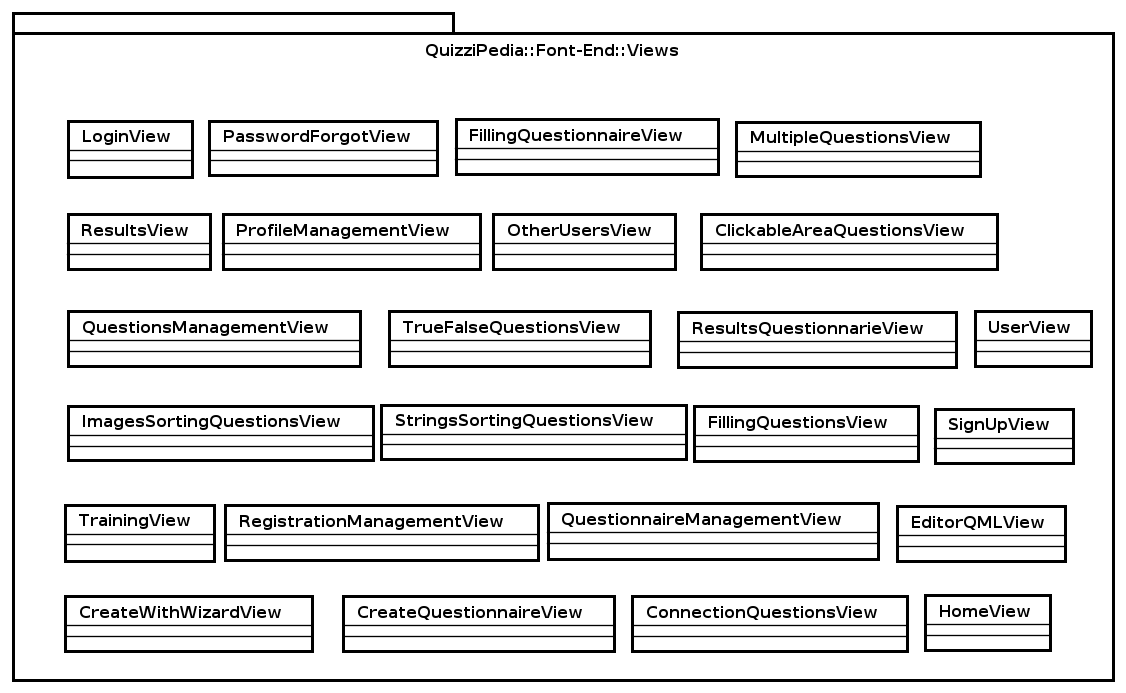
\includegraphics[scale=0.55]{UML/Package/QuizziPedia_Front-End_Views.png}
	\caption{QuizziPedia::Front-End::Views}
\end{figure}\FloatBarrier
\begin{itemize}
	\item \textbf{Descrizione}: package contenente le views front-end dell'applicazione;
	\item \textbf{Padre}: \texttt{Front-End};
	\item \textbf{Interazione con altri componenti}:
	\begin{itemize}
		\item \texttt{Controllers}: package contenente i \textit{controllers\ped{G}} Front-End dell'applicazione;
		\item \texttt{Directives}: package contenente le \textit{directives\ped{G}} Front-End dell'applicazione.
	\end{itemize}
	\item \textbf{Classi contenute}:
	\begin{itemize}
		\item \texttt{LoginView}: classe contenente le form necessarie per effettuare il login. Contiene inoltre un link alla pagina di registrazione e uno alla pagina per il recupero della password;
		\item \texttt{SignUpView}: classe contenente le form dedicate alla registrazione utente. Contiene inoltre un link alla pagina di login;
		\item \texttt{PasswordForgotView}: classe contenente le form necessarie per il recupero della password dimenticata;
		\item \texttt{HomeView}: classe contenente la direttiva per barra di ricerca degli utenti e questionari e il bottone che porterà l'utente nella modalità allenamento;
		\item \texttt{ResultsView}: classe contenente i risultati della ricerca effettuata. Vengono visualizzati sia gli utenti che i questionari trovati;
		\item \texttt{UserView}: contenente le direttive dei dati personali dell'utente, delle sue statistiche relative ai questionari e agli allenamenti effettuati e dei questionari a cui è iscritto;
		\item \texttt{OtherUserView}: classe contenente le direttive dei dati personali e delle statistiche di un utente ricercato;
		\item \texttt{ProfileManagementView}: classe contenente i dati personali che un utente può modificare dopo essersi registrato al sistema;
		\item \texttt{QuestionsManagementView}: classe contenente l'elenco delle domande create;
		\item \texttt{TrueFalseQuestionView}: classe contenente le direttive per creare una domanda vero/falso;
		\item \texttt{MultipleQuestionView}: classe contenente le direttive per creare una domanda a risposta multipla;
		\item \texttt{ConnectionQuestionView}: classe contenente i campi e le direttive per creare una domanda a collegamento;
		\item \texttt{ImagesSortingQuestionView}: classe contenente i campi e le direttive per creare una domanda a ordinamento immagini;
		\item \texttt{StringsSortingQuestionView}: classe contenente i campi e le direttive per creare una domanda a ordinamento stringhe;
		\item \texttt{FillingQuestionsView}: classe contenente i campi e le direttive per creare una domanda a riempimento testo;
		\item \texttt{ClickableAreaQustionView}: classe contenente i campi e le direttive per creare una domanda ad area cliccabile;
		\item \texttt{EditorQMLView}: classe contenente l'editor \textit{QML\ped{G}} per la creazione di domande personalizzate;
		\item \texttt{TrainingView}: classe principale della modalità allenamento; conterrà i vari templates di ogni domanda dell'allenamento;
		\item \texttt{FillingQuestionnaireView}: classe principale per la compilazione del questionario; conterrà i vari templates di ogni domanda appartenente al questionario;
		\item \texttt{QuestionnaireManagementView}: classe principale per la gestione dei questionari;
		\item \texttt{CreateQuestionnaireView}: classe per la creazione del questionario;
		\item \texttt{ResultQuestionnaireView}: classe contenente i risultati conseguiti dagli utenti che hanno compilato il proprio questionario;
		\item \texttt{RegiastrationManagementView}: classe che permette di visualizzare gli utenti iscritti ad un questionario.
	\end{itemize}
\end{itemize}
\newpage
\subsection{QuizziPedia::Front-End::Controllers}

\begin{figure} [ht]
	\centering
	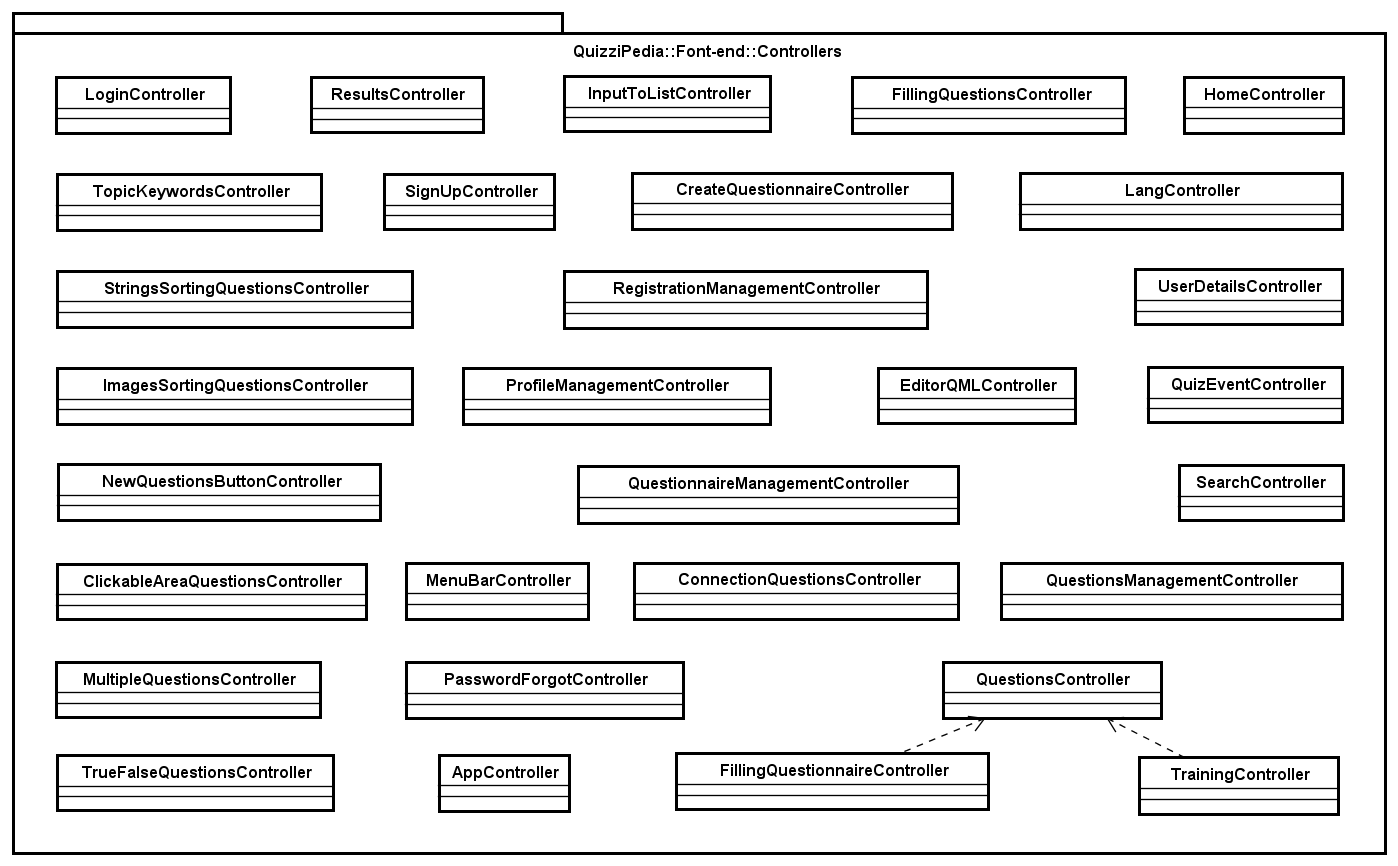
\includegraphics[scale=0.45]{UML/Package/QuizziPedia_Front-End_Controllers.png}
	\caption{QuizziPedia::Front-End::Controllers}
\end{figure} \FloatBarrier

\begin{itemize}
	\item \textbf{Descrizione}: \textit{package\ped{G}} che contiene i controller individuati per la parte front-end dell'applicazione;
	\item \textbf{Padre}: \texttt{Front-End};
	\item \textbf{Interazione con altri componenti}:
	\begin{itemize}
		\item \texttt{Views}: \textit{package\ped{G}} che contiene le \textit{views\ped{G}} dell'applicazione;
		\item \texttt{Models}: \textit{package\ped{G}} che contiene le classi \textit{model\ped{G}} dell'applicazione;
		\item \texttt{Services}: \textit{package\ped{G}} che contiene i \textit{services\ped{G}} dell'applicazione.
	\end{itemize}
	\item \textbf{Classi contenute}:
	\begin{itemize}
		\item \texttt{ClickableAreaQuestionController}: questa classe permette di gestire la creazione e la modifica di una domanda ad area cliccabile;
		\item \texttt{ConnectionQuestionController}: questa classe permette di gestire la creazione e la modifica di una domanda a collegamento;
		\item \texttt{CreateQuesrtionnaireController}: questa classe permette di gestire la creazione di un questionario;
		\item \texttt{EditorQMLController}: questa classe permette di gestire la creazione e la modifica di domande create tramite editor \textit{QML\ped{G}};
		\item \texttt{FillingQuestionnaireController}: questa classe permette di gestire la compilazione del questionario;
		\item \texttt{FillingQuestionsController}: questa classe permette di gestire la creazione e la modifica di una domanda	a riempimento di spazi;
		\item \texttt{HomeController}: questa classe permette di gestire la home page;
		\item \texttt{ImagesSortingQuestionsController}: questa classe permette di gestire la creazione e la modifica di una domanda a ordinamento immagini;
		\item \texttt{InputToListController}: questa classe permette di gestire l'inserimento di una lista di risposte durante la creazione di una domanda;
		\item \texttt{LoginController}: questa classe permette di gestire l'autenticazione dell'utente al sistema;
		\item \texttt{MenuBarController}: questa classe permette di gestire il menù fisso per ogni pagina;
		\item \texttt{MultipleQuestionController}: questa classe permette di gestire la creazione e la modifica di una domanda a risposta multipla;
		\item \texttt{NewQuestionButtonController}: questa classe permette di effettuare il redirect alla pagina di creazione nuova domanda;
		\item \texttt{PasswordForgotController}: questa classe permette di gestire il ripristino della password dimenticata;
		\item \texttt{ProfileManagementController}: questa classe permette di gestire il profilo personale di un utente;
		\item \texttt{QuestionnaireDeatailsController}: questa classe permette di gestire i dettagli di un questionario;
		\item \texttt{QuestionnaireManagementController}: questa classe permette di gestire tutti i questionari creati da un utente;
		\item \texttt{QuestionsController}: questa classe permette di gestire il recupero delle domande per far si che possano essere visualizzate nella modalità allenamento e nella compilazione dei questionari;
		\item \texttt{QuestionsManagementController}: questa classe permette di gestire le domande create dall'utente e di crearne di nuove;
		\item \texttt{QuizEventController}: questa classe permette di reagire ai comandi dell'utente durante la gestione dei suoi questionari;
		\item \texttt{RegistrationManagementController}: questa classe permette di gestire le iscrizione degli utenti ai questionari;
		\item \texttt{ResultQuestionnaireController}: questa classe permette di gestire la visualizzazione dei risultati di un singolo questionario;
		\item \texttt{SearchController}: questa classe permette di gestire la ricerca di questionari e utenti all'interno dell'applicazione;
		\item \texttt{SignUpController}: questa classe permette di gestire la registrazione di un utente al sistema;
		\item \texttt{StatisticsController}: questa classe permette di gestire le statistiche di un utente;
		\item \texttt{StringsSortingQuestionController}: questa classe permette di gestire la creazione e la modifica di una domanda a ordinamento di stringhe;
		\item \texttt{TopicKeywordsController}: questa classe permette di gestire il recupero delle parole chiave di un questionario;
		\item \texttt{TrainingController}: questa classe permette di gestire la modalità allenamento sottoponendo all'utente le giuste domande adatte al suo livello;
		\item \texttt{TrueFalseQuestionController}: questa classe permette di gestire la creazione e la modifica di una domanda	vero/falso;
		\item \texttt{UserDetailsController}: questa classe permette di gestire i dati di un utente da mostrare nella pagina di un profilo.
	\end{itemize} 
\end{itemize}
\newpage
\subsection{QuizziPedia::Front-End::Services}
\begin{figure}[ht]
	\centering
	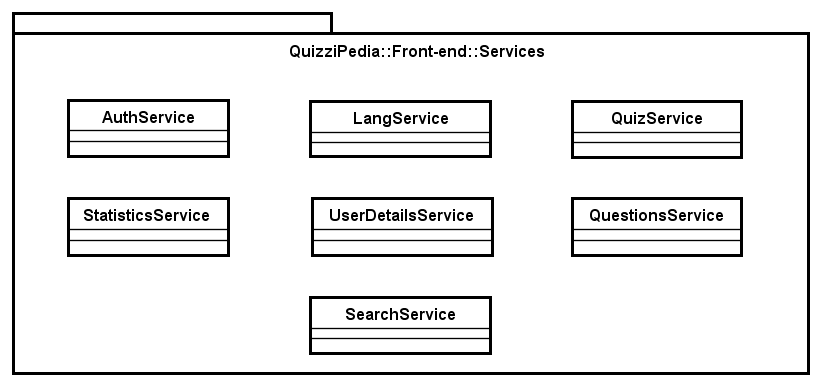
\includegraphics[scale=0.55]{UML/Package/QuizziPedia_Front-End_Services.png}
	\caption{QuizziPedia::Front-End::Services}
\end{figure} \FloatBarrier

\begin{itemize}
	\item \textbf{Descrizione}: package che contiene le classi individuate che permettono la comunicazione del lato front-end con il lato back-end;
	\item \textbf{Padre:} \texttt{Front-End};
	\item \textbf{Interazione con altri componenti:}
	\begin{itemize}
		\item \texttt{Models}: package che contiene le classi \textit{model\ped{G}} dell'applicazione;
		\item \texttt{Controllers}: package che contiene le classi \textit{controller\ped{G}} dell'applicazione.
	\end{itemize}
	\item \textbf{Classi contenute}:
	\begin{itemize}
		\item \texttt{AuthServices}: questa classe permette di gestire la registrazione e l'autenticazione di un utente;
		\item \texttt{LangService}: questa classe permette di gestire la lingua nella quale si è scelto di utilizzare l'applicazione;
		\item \texttt{QuestionsService}: questa classe permette di ottenere domande esistenti e salvare nuove domande;
		\item \texttt{QuizService}: questa classe permette di ottenere i dati di un quiz tramite delle parole chiave inserite dall'utente nella barra di ricerca. Permette inoltre di iscriversi ad un questionario e di scaricare l'intera lista di domande di un questionario a partire dal suo id univoco;
		\item \texttt{SearchService}: questa classe permette di gestire il recupero dei dati dal back-end a seguito di una ricerca effettuata da un utente;
		\item \texttt{StatisticsService}: questa classe permette di ottenere le statistiche dell'utente;
		\item \texttt{UserDetailsService}: questa classe permette di ottenere i dati personali degli utenti.
	\end{itemize} 
\end{itemize}
\newpage

\subsection{QuizziPedia::Front-End::Directives}

\label{QuizziPedia::Front-End::Directives}
\begin{figure} [ht]
	\centering
	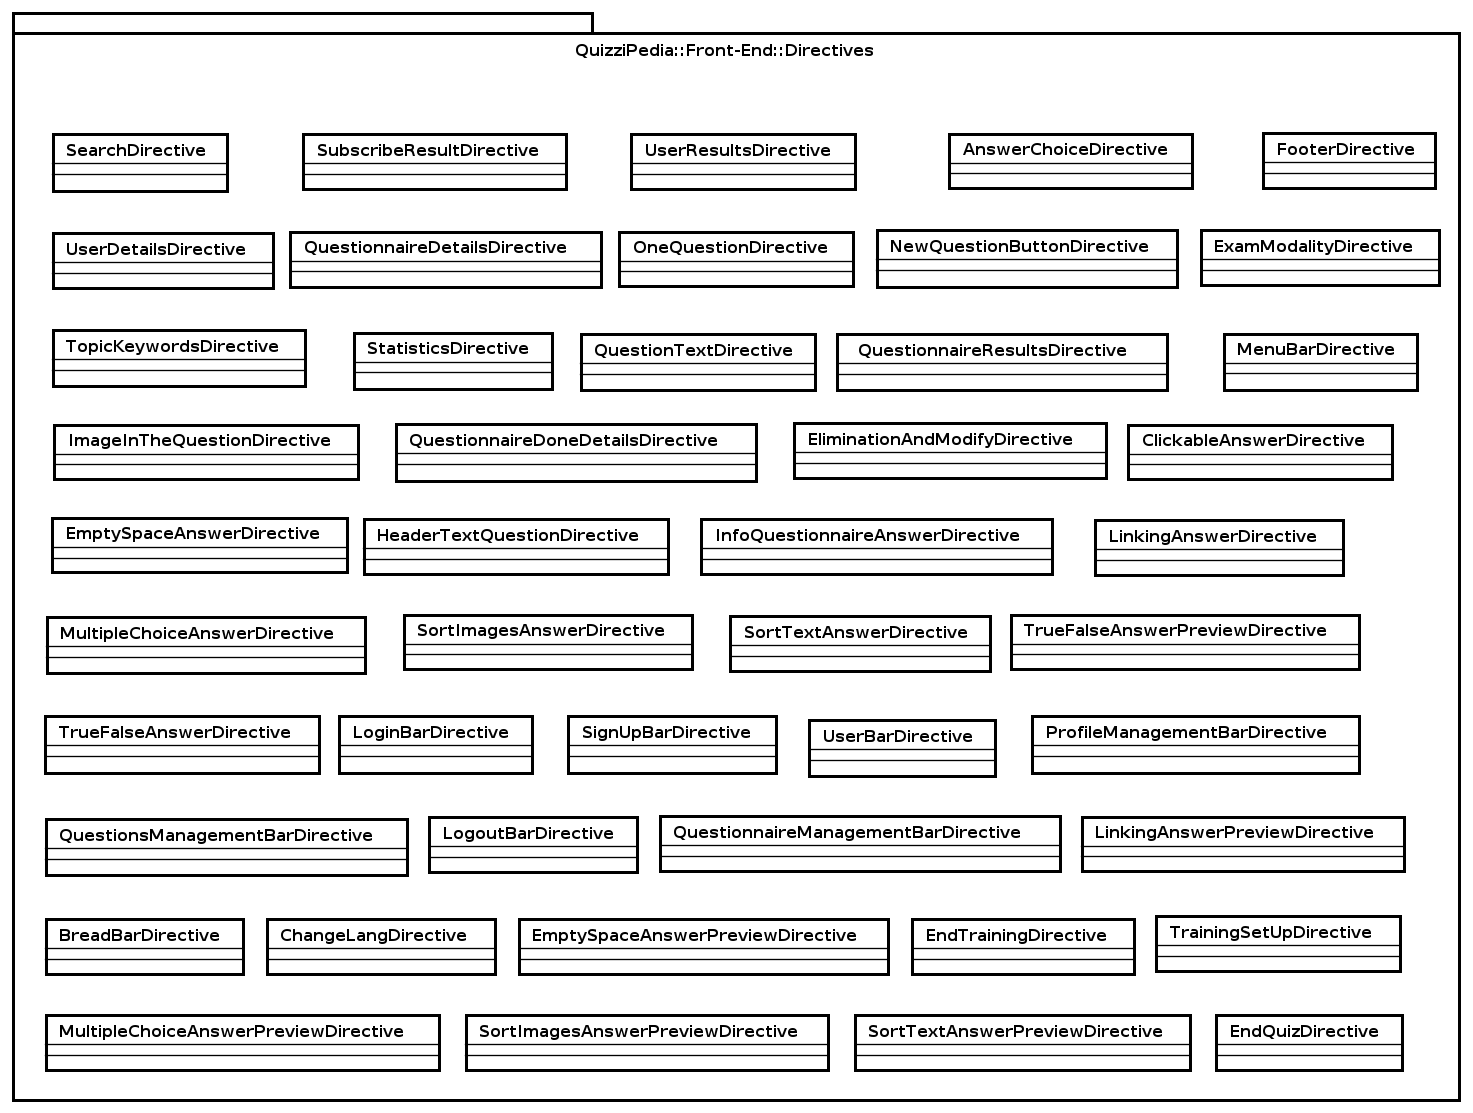
\includegraphics[scale=0.40]{UML/Package/QuizziPedia_Front-End_Directives.png}
	\caption{QuizziPedia::Front-End::Directives}
\end{figure}

\begin{itemize}
	\item \textbf{Descrizione}: package contenente le \textit{directives\ped{G}};
	\item \textbf{Padre}: \texttt{Front-End};
	\item \textbf{Interazione con altri componenti}:
	\begin{itemize}
		\item \texttt{Controllers}: package contenente i \textit{controllers\ped{G}} front-end dell'applicazione;
		\item \texttt{Views}: package contenente le \textit{views\ped{G}} front-end dell'applicazione.
	\end{itemize}
	\item \textbf{Classe contenute}:
	\begin{itemize}
		\item \texttt{EliminationAndModifyDirective}: componente grafico contenente i bottoni per eliminare o modificare un questionario;
		\item \texttt{ExamModalityDirective}: classe contenete i componenti grafici per attivare la modalità esame su un questionario e gestire le iscrizioni;
		\item \texttt{FooterDirective}: classe contenente i componenti grafici del footer dell'applicazione;
		\item \texttt{ImageInTheQuestionDirective}: classe contenente i componenti grafici per l'inserimento dell'immagine	nella creazione delle domande;
		\item \texttt{MenuBarDirective}: rappresenta il menù, presente in ogni pagina dell'applicazione, generato in base agli oggetti passati nello \$scope isolato. Fornisce un pulsante per ogni oggetto ricevuto come parametro, ogni pulsante viene rappresentato con un'icona e con un testo. Al click di un pulsante viene invocata la funzione ad esso associata;
		\item \texttt{OneQuestionDirective}: rappresenta il componente grafico che visualizza all'utente l'anteprima della domanda che ha creato. Eseguendo l'azione di click sul pulsante di modifica sarà possibile modificare tale domanda. All'interno di QuestionsManagementsView verranno stampati a video tanti componenti quanti presenti nello \$scope isolato ad esso associato;
		\item \texttt{NewQuestionButtonDirective}: rappresenta il componente grafico che permette all'utente di posizionarsi nella \textit{view\ped{G}} di creazione di una nuova domanda;
		\item \texttt{QuestionTextDirective}: rappresenta il componente grafico che permette all'utente di scrivere o modificare il testo di una domanda;
		\item \texttt{QuestionnaireDetailsDirective}: rappresenta il componente grafico che permette all'utente di visualizzare la lista di questionari che può compilare;
		\item \texttt{QuestionnaireDoneDetailsDirective}: rappresenta il componente grafico che permette all'utente di visualizzare la lista di questionari che ha già compilato e di conseguenza vederne le valutazioni;
		\item \texttt{QuestionnaireResultsDirective}: rappresenta il componente grafico che permette all'utente autenticato pro di vedere i risultati di chi ha compilato il questionario. Tale componente è contenuto nella lista dei questionari abilitati alla compilazione. É possibile accedere alla lista dei risultati azionando l'evento ad esso collegato;
		\item \texttt{QuestionnaireResultsDirective}: rappresenta il componente grafico che permette all'utente autenticato pro di vedere i risultati di chi ha compilato il questionario. Tale componente è contenuto nella lista dei questionari abilitati alla compilazione. É possibile accedere alla lista dei risultati azionando l'evento ad esso collegato;
		\item \texttt{SearchDirective}: classe che permette di effettuare la ricerca di utenti e questionari;
		\item \texttt{StatisticsDirective}: classe che permette di visualizzare le statistiche di un utente;
		\item \texttt{SubscribeResultDirective}: classe che permette di visualizzare e iscriversi ai questionari ricercati;
		\item \texttt{TopicKeywordsDirective}: classe che permette di gestire l'inserimento dell'argomento e delle	keywords al momento della creazione della domanda;
		\item \texttt{UserDetailsDirective}: classe che permette di visualizzare i dati personali di un utente;
		\item \texttt{UserResultsDirective}: classe che permette di visualizzare la lista degli utenti ricercati dopo aver utilizzato l'apposita funzione di ricerca;
		\item \texttt{ClickableAnswerDirective}: rappresenta il componente grafico che permette all'utente di visualizzare la domanda ad area cliccabile nell'immagine;
		\item \texttt{EmptySpaceAnswerDirective}: rappresenta il componente grafico che permette all'utente di visualizzare l'esercizio a riempimento di spazi vuoti;
		\item \texttt{HeaderTextQuestionDirective}: rappresenta componente grafico che presenta all'utente l'argomento e le parole chiave della domanda che ha a schermo;
		\item \texttt{InfoQuestionnaireDirective}: rappresenta il componente grafico che permette all'utente di visualizzare le informazioni principali del questionario che si sta per svolgere;
		\item \texttt{LinkingAnswerDirective}: rappresenta componente grafico che permette all'utente di visualizzare la domanda di collegamento;
		\item \texttt{MultipleChoiceAnswerDirective}: rappresenta componente grafico che permette all'utente di visualizzare la domanda a risposta multipla;
		\item \texttt{SortImagesAnswerDirective}: rappresenta il componente grafico che permette all'utente di visualizzare la domanda ad ordinamento di immagini;
		\item \texttt{SortTextAnswerDirective}: rappresenta il componente grafico che permette all'utente di visualizzare la domanda ad ordinamento di stringhe;
		\item \texttt{TrainingSetUpDirective}: rappresenta componente grafico che permette all'utente di selezionare l'argomento e le parole chiave per iniziare un allenamento con queste caratteristiche;
		\item \texttt{TrueFalseAnswerDirective}: rappresenta il componente grafico che permette all'utente di visualizzare la domanda vero e falso;
		\item \texttt{LoginBarDirective}: directive contenente il componente che permette di effettuare il redirect alla pagina di login;
		\item \texttt{SignUpBarDirective}: directive contenente il componente che permette di effettuare il redirect alla pagina di registrazione;
		\item \texttt{UserBarDirective}: directive contenente il componente che permette di effettuare il redirect alla pagina di visualizzazione profilo;
		\item \texttt{ProfileManagementBarDirective}: directive contenente il componente che permette di effettuare il redirect alla pagina di gestione del profilo;
		\item \texttt{QuestionsManagementBarDirective}: directive contenente il componente che permette di effettuare il redirect alla pagina di gestione delle domande;
		\item \texttt{LogoutBarDirective}: directive contenente il componente che permette di effettuare il logout dal sistema;
		\item \texttt{QuestionnaireManagementBarDirective}: directive contenente il componente che permette di effettuare il redirect alla pagina di gestione dei questionari.
	\end{itemize}
\end{itemize}
\newpage

\subsection{QuizziPedia::Front-End::Models}

	\label{QuizziPedia::Front-End::Models}
	
	\begin{figure}[ht]
		\centering
		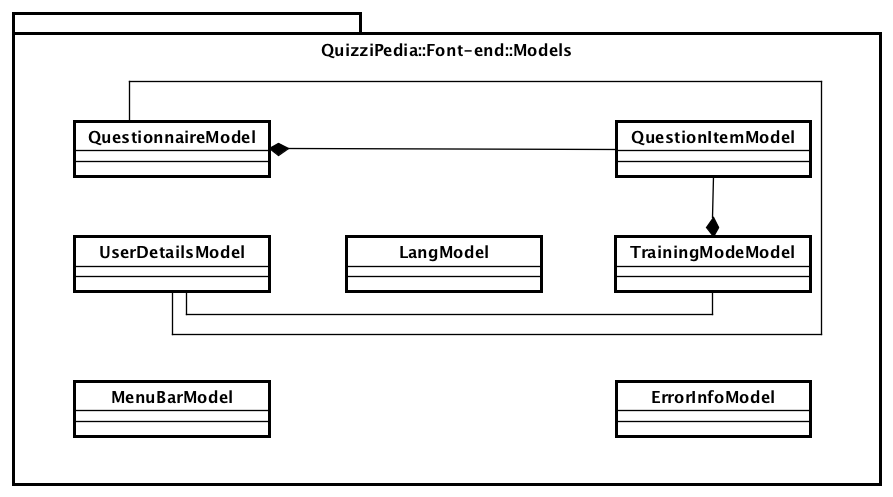
\includegraphics[scale=0.5,keepaspectratio]{UML/Package/QuizziPedia_Front-End_Models.png}
		\caption{QuizziPedia::Front-End::Models}
	\end{figure} \FloatBarrier

		\begin{itemize}
			\item \textbf{Descrizione}: \textit{package\ped{G}} contenente le classi che definiscono la business logic dell'applicazione;
			\item \textbf{Padre}: \texttt{Front-End};
			\item \textbf{Iterazioni con altri componenti}: 
				\begin{itemize}				
					\item \texttt{Controllers}: \textit{package\ped{G}} contenente i controllers front-end dell'applicazione;
					\item \texttt{Directives}: \textit{package\ped{G}} contenente le directives front-end dell'applicazione;
					\item \texttt{Models}: \textit{package\ped{G}} contenente le classi che definiscono la business logic dell'applicazione;
					\item \texttt{Services}: \textit{package\ped{G}} che contiene le classi individuate che permettono la comunicazione del lato front-end con il lato back-end attraverso l'architettura \textit{REST\ped{G}}.
				\end{itemize}
			\item \textbf{Classi contenute}:
			\begin{itemize}
				\item \texttt{UserDetailsModel}: rappresenta un utente. Contiene tutte le informazioni necessarie alla presentazione del contenuto di un utente sia nella visualizzazione che nella gestione di un profilo;
				\item \texttt{TrainingModeModel}: rappresenta un allenamento. Contiene tutte le informazioni necessarie alla presentazione del contenuto di un allenamento;
				\item \texttt{QuestionnaireModel}: rappresenta un questionario. Contiene tutte le informazioni necessarie alla presentazione del contenuto del questionario;
				\item \texttt{QuestionItemModel}: rappresenta una domanda. Contiene tutte le informazioni necessarie alla presentazione del contenuto della domanda;
				\item \texttt{MenuBarModel}: questa classe racchiude i dati necessari per la creazione dinamica della barra menù posizionata in modo fisso su ogni pagina;
				\item \texttt{LangModel}: rappresenta le informazioni per la giusta traduzione dell'applicazione;
				\item \texttt{ErrorInfoModel}: rappresenta le informazioni di un errore che si è verificato eseguendo una determinata operazione;
			\end{itemize}
		\end{itemize}
